\section{Relatività Ristretta}\label{sec:1}
\subsection{Basi filosofiche della Relatività Ristretta}
La meccanica classica nasce attraverso un lungo e geniale processo di razionalizzazione dei concetti che, intuitivamente, la nostra ragione ci suggerisce: lo spazio è il luogo dove i corpi si trovano e si muovono, il tempo è il concetto che ci consente di scandire la successione dei fenomeni o, ancora, la forza è il modo in cui abbiamo razionalizzato l'interazione tra gli oggetti, ecc. A tutto questo si accompagna la formulazione, ossia la necessità di rendere la relazione tra i concetti quantitativa, che viene rappresentata -in ultima analisi- dalle equazioni differenziali; come scrive Poincaré all'inizio del decimo capitolo di \textit{La scienza e l'ipotesi}: \say{Le equazioni differenziali sono sempre vere, [...]; queste equazioni esprimono relazioni e se le equazioni rimangono vere è perché le relazioni conservano la loro realtà}. Oppure ancora: \say{Le vere relazioni tra questi oggetti reali sono l'unica realtà che possiamo raggiungere, e l'unica condizione è che esistano tra questi oggetti le stesse relazioni che esistono tra le immagini che siamo costretti a mettere al loro posto}.\\
Possiamo dunque, pensare la meccanica classica come un potente raffinamento delle idee quotidiane ed una sorprendente capacità di mettere in formule le relazioni fra i concetti che, si assume, corrispondano agli oggetti reali.

Un primo concetto, di fondamentale importanza, in meccanica classica è il sistema di riferimento, caratterizzato come una terna di rette perpendicolari che rappresenta lo spazio di un osservatore. Risulta evidente come ad osservatori diversi siano associabili diversi sistemi di riferimento e da ciò segue che il moto di questi, potrà, in generale, essere vario. Una categoria rilevante, nello studio meccanico, di sistemi di riferimento è quella individuata come sistemi di riferimento inerziali, ovvero quei sistemi il cui moto risulta essere rettilineo uniforme.
Una volta chiarita questa struttura concettuale è immediato comprendere la natura relativa dello spazio, mentre il tempo -nel contesto classico- viene considerato assoluto. Vale a dire che la progressione temporale risulta coerente per tutti i sistemi di riferimento. La rilevanza dei sistemi inerziali è dovuta al principio di relatività galileiano, il quale afferma: le leggi della meccanica sono invarianti, in forma, in tutti i sistemi di riferimento inerziali. Ciò che, di fatto, si assume con questo principio è l'equivalenza tra i diversi sistemi di riferimento. Questo garantisce la coerenza delle osservazioni, ovvero -ai fini di uno studio scientifico- è necessario assumere che le realtà fenomenologiche di osservatori diversi siano coese in modo da formare un'unica realtà che, attraverso i successi della fisica classica, è ritenuta oggettiva. Perché questo sia garantito è necessario ipotizzare che le relazioni tra le quantità -come detto le equazioni differenziali- siano assolute\footnote{Almeno nel regime inerziale considerato dal principio.}.\\
Lo sviluppo teorico della meccanica classica mostra come, storicamente, sia stata fatta un'altra assunzione, ossia che le interazioni naturali dispongano di una velocità infinita. Tuttavia, l'esperienza ha abbondantemente dimostrato che, nella natura macroscopica, non esistono interazioni istantanee. Questa rappresenta una prima imprecisione della meccanica classica, la quale è stata il primo punto di superamento che la teoria della relatività ristretta ha compiuto rispetto alla teoria precedente. 
Difatti, la teoria della relatività riprende -seppur ampliandolo a tutti i fenomeni fisici- il principio di relatività e postula, inoltre, l'invarianza della velocità della luce \textit{\textbf{c}} rispetto a tutti i sistemi di riferimento inerziali. Questo secondo postulato porta all'inevitabile risultato di porre la velocità della luce come velocità limite.
Chiariamo come le due cose siano correlate; consideriamo un primo sistema di riferimento in quiete ed un secondo sistema in moto rettilineo uniforme, a questo punto consideriamo un oggetto che si muove a una determinata velocità in verso opposto al sistema di riferimento in moto. \`E chiaro come la velocità dell'oggetto misurata dal sistema in moto risulterà superiore rispetto a quella misurata dal sistema in quiete. Ora, immaginiamo di accelerare l'oggetto fino alla velocità della luce, quando l'oggetto la raggiungerà -per il postulato- la misura dei due sistemi di riferimento sarà la medesima. Aggiungiamo un terzo sistema di riferimento, che si muove con una velocità doppia rispetto al secondo e nella stessa direzione; anche per questo l'oggetto andrà alla velocità della luce. Risulta chiaro come il postulato vieti l'esistenza di un sistema di riferimento per il quale l'oggetto superi la velocità della luce, divenendo questa un limite. 

Pertanto, il principio di relatività einsteiniano affiancato dal postulato dell'esistenza di una velocità limite, formano la base teoretica della relatività ristretta.\\
Anche assumendo che l'interazione viaggi alla velocità massima, risulta evidente come una velocità finita di trasmissione del realizzarsi di un fenomeno, metta in crisi il concetto di simultaneità della fisica pre-relativistica, fondato, a sua volta, sul concetto di tempo assoluto.\\
Siamo, dunque, giunti ad una contraddizione tra l'impianto filosofico della relatività ristretta e l'idea classica di tempo assoluto. Per proseguire è necessario negare una delle due ipotesi.
Procediamo negando il carattere assoluto del tempo e facendolo diventare un concetto relativo, al pari dello spazio in meccanica classica.
In questo modo, tuttavia, siamo usciti dalla meccanica classica, infatti l'assunzione che il tempo sia relativo esce dalla nostra concezione quotidiana del mondo, sulla quale -come detto- si basa la fisica classica, causando, in maniera del tutto propria, un cambio di paradigma.
\subsection{Trasformazioni di Lorentz}\label{sec:1.1}
Come detto nella sezione precedente la teoria della relatività ristretta pone come punto di partenza due postulati:
\begin{enumerate}
    \item il \textit{principio di relatività};
    \item il \textit{principio di invarianza della velocità della luce}.
\end{enumerate}

Ora vogliamo definire delle trasformazioni che, risultando compatibili con i due postulati, leghino le coordinate spaziotemporali di due sistemi di rifermento inerziali.
Più precisamente, per via del secondo postulato, vogliamo che le equazioni di Maxwell -le quali descrivono la propagazione della luce- risultino invarianti per la trasformazione T.

\begin{figure}[h]
    \centering
    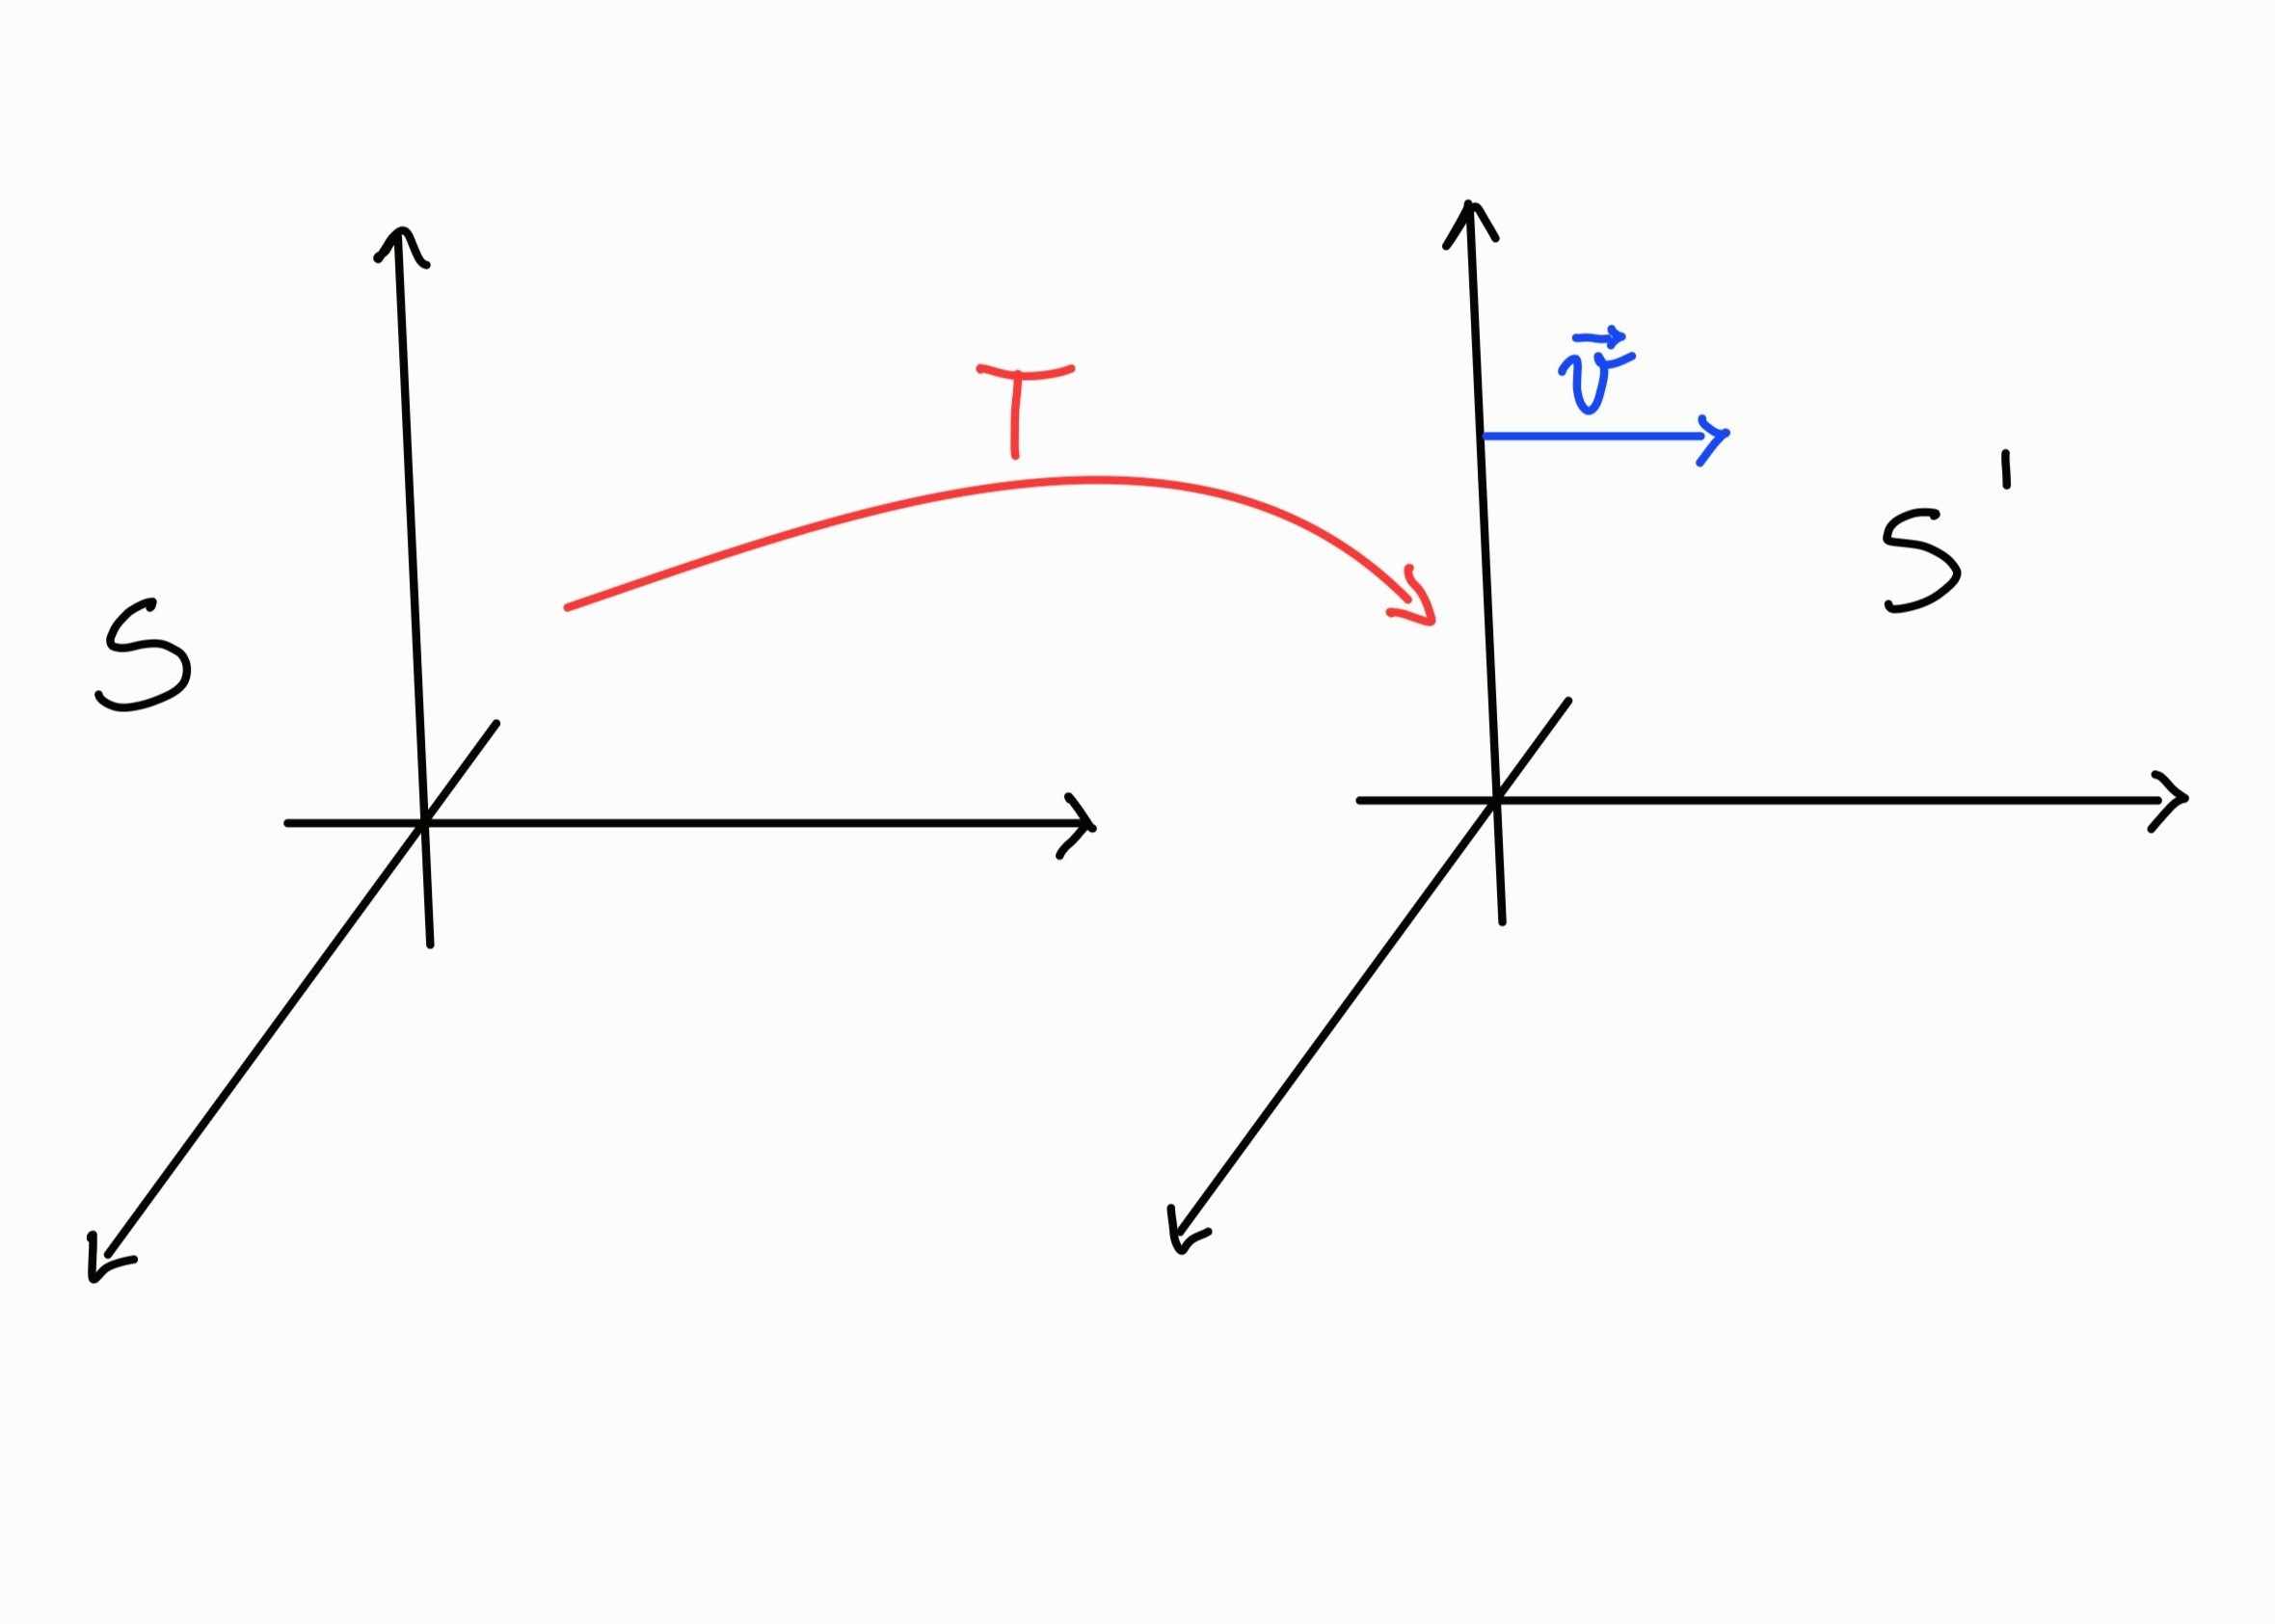
\includegraphics[width=0.40\textwidth]{Immagini/Tras_Lorentz.jpg}
    \caption{ $T : S \rightarrow{} S'$}
    \label{fig:TL}
\end{figure}
La trasformazione che stiamo cercando dovrà essere necessariamente lineare, questo perché il moto considerato è rettilineo uniforme, ovvero:

\begin{equation}
    \begin{cases}
      \dfrac{d^2\vec{x}}{{dt}^2}=0
             \\
     \dfrac{d^2\Vec{x'}}{{dt}^2}=0
    \end{cases}\,
\end{equation}

Definiamo, ora, un \textit{evento} come un vettore, contravariante\footnote{Analizzeremo, in maniera approfondita, questo concetto più avanti.}, quadridimensionale del tipo:

\begin{equation}\label{eq:def_evento}
  x^{\alpha}=(x^0,x^1,x^2,x^3)=(ct, \Vec{x})=(ct,x,y,z)
\end{equation}
quindi la trasformazione lineare possiamo scriverla come:


\begin{equation}
  x^{\alpha}\xrightarrow[\text{}]{\text{T}}x'^{\beta}=\Lambda\indices{^\beta_\nu} x^{\nu}
\end{equation}
In questa notazione si è fatto uso della convenzione di Einstein. Quindi, per maggiore chiarezza, se fissiamo $ \beta=0 $ si ha che:
\begin{equation*}
  x'^{0}=ct'=\Lambda\indices{^0_0}x^0+\Lambda\indices{^0_1}x^1+\Lambda\indices{^0_2}x^2+\Lambda\indices{^0_3}x^3     \qquad   \forall\alpha=0,1,2,3
\end{equation*}

Le trasformazioni lineari che soddisfano i postulati della relatività ristretta sono le \textit{trasformazioni di Lorentz}\footnote{Le trasformazioni di Lorentz sono un caso particolare delle trasformazioni di Poincaré.}.

Consideriamo il sistema di riferimento $S'$ in moto rispetto al sistema $S$ con velocità costante $\Vec{v}$ lungo la sola direzione x, come mostrato in Fig.\ref{fig:TL}. 
\newpage
Definiamo, allora, le quantità:

\begin{equation}
    \begin{cases}
      \beta=\dfrac{v}{c}
             \\
     \gamma = \dfrac{1}{\sqrt{1-\dfrac{v^{2}}{c^{2}}}}
    \end{cases}\,
\end{equation}
dunque le trasformazioni di Lorentz sono della forma:

\begin{equation}
    \begin{cases}
      ct'=\dfrac{ct-\beta x}{\sqrt{1-\beta^2}}
             \\
     x' = \dfrac{x-vt}{\sqrt{1-\beta^2}}
    \end{cases}\,
\end{equation}
Considerando la natura quadridimensionale di un evento avremo che la matrice di trasformazione avrà sedici elementi

\begin{equation}\label{eq:def_trasf}
\Lambda(\beta)\equiv
\{\Lambda\indices{^\mu_\nu}\}=
\{ \dfrac{\partial x'^\mu}{\partial x^\nu} \}=
\begin{pmatrix}
\Lambda\indices{^0_0} & \Lambda\indices{^0_1}& \Lambda\indices{^0_2} & \Lambda\indices{^0_3}   \\
\Lambda\indices{^1_0} & \Lambda\indices{^1_1}& \Lambda\indices{^1_2} & \Lambda\indices{^1_3}  \\
 \Lambda\indices{^2_0} & \Lambda\indices{^2_1}& \Lambda\indices{^2_2} & \Lambda\indices{^2_3}               \\
  \Lambda\indices{^3_0} & \Lambda\indices{^3_1}& \Lambda\indices{^3_2} & \Lambda\indices{^3_3}
\end{pmatrix}\footnote{Si noti che, nella notazione tensoriale, l'indice più esterno rappresenta la colonna, mentre quello più interno rappresenta la riga.}
\end{equation}
 La matrice associata alla trasformazione lineare sarà simmetrica e avrà forma: 
\begin{equation}
\Lambda(\beta)=
\begin{pmatrix}
\gamma & -\gamma\beta & 0 & 0   \\
 -\gamma\beta &\gamma & 0 & 0    \\
  0 & 0 & 1 & 0                   \\
  0 & 0 & 0 & 1
\end{pmatrix}
\end{equation}
In generale se il moto del sistema $S'$ non è parallelo ad una sola direzione allora gli elementi della matrice assumono la forma:
\begin{equation}\phantomsection\label{eq:generic_elem_tras}
    \begin{gathered}
    \Lambda\indices{^0_0}=\gamma;  \quad   \Lambda\indices{^0_i}=\Lambda\indices{^i_0}=-\beta_i\gamma;\\
     \Lambda\indices{^i_j}=\delta_{ij}+\dfrac{(\gamma-1)}{\beta^2}\beta_i\beta_j\qquad   \forall i,j=1,2,3
\end{gathered}
\end{equation}

ove $\delta_{ij}$ è la delta di Kronecker.

Definiamo la forma quadratica ${ds}^2=c^2{dt}^2-{dx}^2-{dy}^2-{dz}^2$, la quale prende il nome di \textit{intervallo}.
Possiamo scrivere la forma quadratica in maniera molto compatta utilizzando il formalismo tensoriale:
\begin{equation}\label{Eq:def_int}
  {ds}^2=\eta\indices{_{ij}}dx^idx^j
\end{equation}
ove $\eta\indices{_{ij}}$ sono gli elementi della matrice:
\begin{equation} \label{Eq:def_eta}
\eta=
\begin{pmatrix}
  1 & 0 & 0 & 0  \\
  0 & -1 & 0 & 0  \\
  0 & 0 & -1 & 0   \\
  0 & 0 & 0 & -1
\end{pmatrix}
\end{equation}
ed $\eta$ è detto \textit{tensore metrico}.

Possiamo ridefinire, più formalmente, la trasformazione di Lorentz come una trasformazione lineare i cui elementi soddisfano la seguente relazione di invarianza\footnote{Anche qui, come in avanti, si è utilizzata la convenzione di Einstein. Senza sottintendere le sommatorie avremmo: $\sum_{\alpha=1}^{4}\sum_{\beta=1}^{4}\eta\indices{_{\alpha \beta}}\Lambda\indices{^\alpha_\mu}\Lambda\indices{^\beta_\nu}=\eta\indices{_{\mu \nu}}$.}:

\begin{equation}\label{Eq:rel_inv}
\eta\indices{_{\alpha \beta}}\Lambda\indices{^\alpha_\mu}\Lambda\indices{^\beta_\nu}=\eta\indices{_{\mu \nu}}
\end{equation}
Ora dimostriamo che se $\Lambda$ soddisfa la \eqref{Eq:rel_inv}, allora ${ds}^2$ è un invariante per tutti i sistemi di riferimento inerziali.

\begin{proof}
\begin{equation*}
    {ds'}^2=\eta\indices{_{\alpha \beta}}dx'^\alpha dx'^\beta=\eta\indices{_{\alpha \beta}}\Lambda\indices{^\alpha_\mu}\Lambda\indices{^\beta_\nu}dx^\mu dx^\nu=\eta\indices{_{\mu \nu}}dx^\mu dx^\nu={ds}^2
\end{equation*}
\end{proof}


Possiamo riscrivere la relazione di invarianza (trasponendo una matrice\footnote{Nell'operazione di trasposizione si ha l'inversione di righe e colonne, quindi, per rispettare il formalismo, si deve posporre l'indice alto, rispetto a quello basso.}) nella forma:

\begin{equation}
\Lambda\indices{^T_\mu^\alpha}\eta\indices{_{\alpha \beta}}\Lambda\indices{^\beta_\nu}=\eta\indices{_{\mu \nu}}
\end{equation}
che in forma matriciale si scrive:
\begin{equation}
\Lambda\indices{^T}\eta\Lambda=\eta
\end{equation}

Ora, consideriamo i determinanti:
\begin{gather*}
    \det(\Lambda\indices{^T}\eta\Lambda)=\det\eta   \\
\det\Lambda\indices{^T}\det\eta\det\Lambda =\det\eta \\
(\det\Lambda)^2=1\implies \det\Lambda=\pm1
\end{gather*}

Definiamo \textit{trasformazioni proprie} quelle che hanno $\det\Lambda=1$ e \textit{trasformazioni improprie} quelle che hanno $\det\Lambda=-1$.

Ora, ci domandiamo quanti dei $4\times4=16$ elementi della matrice $\Lambda$ siano parametri liberi. Al numero massimo dobbiamo, ovviamente, sottrarre il numero di condizioni che imponiamo, l'unica relazione che abbiamo imposto è la \eqref{Eq:rel_inv}, questa, in linea di principio, comporta $16$ equazioni a causa della doppia sommatoria. Tuttavia, ricordando la definizione di $\eta$ \eqref{Eq:def_eta} si nota che questa è simmetrica, quindi le equazioni indipendenti saranno $10$.
Si conclude così che i parametri liberi sono $16-10=6$. Questo risultato torna fisicamente, poiché i parametri liberi saranno le $3$ direzioni di moto più i $3$ angoli di rotazione del sistema $S'$.

Possiamo fare un ulteriore classificazione delle trasformazioni di Lorentz. Nella relazione \eqref{Eq:rel_inv} abbiamo gli indici $\mu$ e $\nu$ liberi, ponendoli entrambi pari a zero otteniamo:
\begin{equation*}
\eta\indices{_{\alpha \beta}}\Lambda\indices{^\alpha_0}\Lambda\indices{^\beta_0}=\eta\indices{_{00}}=1
\end{equation*}
sviluppando la somma su $\alpha,\beta$ e ricordando che $\eta$ è diagonale, con $\eta\indices{_{11}}=\eta\indices{_{22}}=\eta\indices{_{33}}=-1$, abbiamo:
\begin{gather*}
   \eta\indices{_{00}}(\Lambda\indices{^0_0})^2+\sum_{i=1}^{3}\eta\indices{_{ii}}(\Lambda\indices{^i_0})^2=1   \\
\eta\indices{_{00}}(\Lambda\indices{^0_0})^2=1 +\sum_{i=1}^{3}(\Lambda\indices{^i_0})^2\geq 1 \\
\implies \Lambda\indices{^0_0}\geq 1 \quad \vee   \quad\Lambda\indices{^0_0}\leq -1
\end{gather*}
Allora, definiamo \textit{trasformazioni ortocrone} quelle che hanno $\Lambda\indices{^0_0}\geq 1$ e \textit{trasformazioni non ortocrone} quelle che hanno $\Lambda\indices{^0_0}\leq -1$.


\subsection{Spazio di Minkowski}\label{sec:1.2}
Nella sezione precedente abbiamo definito un evento \eqref{eq:def_evento}, è possibile vedere tale oggetto come un punto in una varietà quadridimensionale, che chiamiamo \textit{spazio di Minkowski}. In tale spazio è definibile un intervallo \eqref{Eq:def_int} invariante rispetto alle trasformazioni di Lorentz.

Facciamo un piccolo esercizio per fissare le idee.

Consideriamo una particella (massiva) in un determinato evento $x^{\alpha}=(ct,x,y,z)$ e dopo un tempo $dt$ infinitesimo si trova nell'evento $x^{\beta}=(c(t+dt),x+dx,y+dy,z+dz)$. Allora l'intervallo associato sarà:
\begin{equation*}
    {ds}^2=c^2{dt}^2-{d\vec{x}}^2>0
\end{equation*}
il termine ${d\vec{x}}^2$ rappresenta lo spazio percorso dalla particella, mentre il termine $c^2{dt}^2$ rappresenta lo spazio che avrebbe percorso la luce nello stesso tempo infinitesimo $dt$. Poiché sappiamo che la velocità della luce è la \textit{velocità limite}\footnote{Questo fatto è sostenuto da dati sperimentali.} la sottrazione dovrà risultare positiva. Inoltre essendo la particella massiva per definizione, allora essa non potrà raggiungere tale velocità, dunque la sottrazione risulta strettamente maggiore di zero.
In generale possiamo distinguere gli intervalli dal loro segno:
\begin{enumerate}
    \item ${ds}^2>0$  l'intervallo è di \textit{genere tempo} (o \textit{time-like}). In tal caso è ammesso che gli eventi considerati abbiano una relazione di causalità;
    \item ${ds}^2=0$ l'intervallo è di \textit{genere luce} (o \textit{light-like}). \`E l'intervallo tipico della luce;
    \item ${ds}^2<0$ l'intervallo è di \textit{genere spazio} (o \textit{space-like}). In questo caso non è ammessa causalità tra gli eventi considerati, poiché il contrario implicherebbe il superamento della velocità limite.
\end{enumerate}
 Il fatto che la velocità della luce sia la velocità limite, dota lo spazio di Minkowski di una \textit{struttura causale}, rappresentata in Fig.\ref{Fig:SM}.
 
\begin{figure}[H]
        \begin{center}
        
     \begin{tikzpicture}[scale=1.8]
  \message{Light cone^^J}
  
  \def\xmax{2}
  \def\xmaxp{2.2} % maximum of rotated axis
  \def\Nlines{5} % number of world lines (at constant x/t)
  \pgfmathsetmacro\d{0.9*\xmax/\Nlines} % grid size
  \pgfmathsetmacro\ang{-atan(1/3)} % angle between x and x' axes
  
  \pgfmathsetmacro\D{2*\d} % distance between observers
  \coordinate (B) at (\D,0); % observer B at t=0
  \coordinate (C) at (45:{\D*sqrt(2)/(1-cot(\ang))});

  \coordinate (O) at (0,0);
  \coordinate (X) at (\xmax+0.2,0);
  \coordinate (T) at (0,\xmax+0.2);
  
  % WORLD LINE GRID
  \message{  Making world lines...^^J}
  \foreach \i [evaluate={\x=\i*\d;}] in {1,...,\Nlines}{
    \message{  Running i/N=\i/\Nlines, x=\x...^^J}
    \draw[world line]   (-\x,-\xmax) -- (-\x,\xmax);
    \draw[world line]   ( \x,-\xmax) -- ( \x,\xmax);
    \draw[world line t] (-\xmax,-\x) -- (\xmax,-\x);
    \draw[world line t] (-\xmax, \x) -- (\xmax, \x);
  }
  
  % AXES
  \draw[->,thick] (0,-\xmax) -- (T) node[left=-1] {$ct$};
  \draw[->,thick] (-\xmax,0) -- (X) node[below=0] {$x$};
  
  % LABELS
  \draw pic[->,"$45^\circ$",draw=black,angle radius=23,angle eccentricity=1.38] {angle = X--O--C};
  

  
  % FILLS
  
  \fill[myblue,opacity=0.05] % TIMELIKE
   (\xmax,\xmax) -- (0,0) -- (-\xmax,\xmax)-- cycle;
    \fill[myred,opacity=0.05] % TIMELIKE
    (-\xmax,-\xmax) -- (0,0) -- (\xmax,-\xmax)-- cycle;
  \node[black,right,align=center] at (-\xmax,0.18*\xmax)
    {\contour{black!5}{Presente}};
  \node[black,left,align=center] at (\xmax,0.18*\xmax)
    {\contour{black!5}{Presente}};
  \node[mydarkblue,align=center] at (-0.22*\xmax,0.67*\xmax)
    {\contour{myblue!5}{Futuro}\\[-2]\contour{myblue!5}{assoluto}};
  \node[myred,align=center] at (0.22*\xmax,-0.67*\xmax)
    {\contour{myorange!5}{Passato}\\[-2]\contour{myorange!5}{assoluto}};
  
  % PHOTON

  \draw[photon] (-\xmax,-\xmax)  -- ( \xmax,\xmax);
    
  \draw[photon] (\xmax,-\xmax) -- (-\xmax,\xmax);
  
  % PARTICLE WORLDLINE
  \draw[particle,decoration={markings,mark=at position 0.27 with {\arrow{latex}},
                                      mark=at position 0.76 with {\arrow{latex}}},postaction={decorate}]
      (-0.5*\xmax,-\xmax) to[out=80,in=-110] (O) to[out=70,in=-100] (0.45*\xmax,\xmax);
  \fill[mydarkgreen] (O) circle(0.04); % event
\end{tikzpicture}
        \caption{\small \textit{Spazio di minkowski}}
        \label{Fig:SM}
        \end{center}
    \hfill
\end{figure}


Consideriamo, ora, due eventi $A=(ct_1,x_1,y_1,z_1)$ e $B=(ct_2,x_2,y_2,z_2)$, allora l'intervallo associato sarà:
\begin{equation*}
    {\Delta s_{AB}}^2=c^2(t_2-t_1)^2-(x_2-x_1)^2-(y_2-y_1)^2-(z_2-z_1)^2=c^2{\Delta t}^2-{\Delta l}^2
\end{equation*}
Gli stessi due eventi, in un altro sistema di riferimento, appaiono come $A'=(ct'_1,x'_1,y'_1,z'_1)$ e $B'=(ct'_2,x'_2,y'_2,z'_2)$, quindi l'intervallo sarà:
\begin{equation*}
    {\Delta s'_{A'B'}}^2=c^2(t'_2-t'_1)^2-(x'_2-x'_1)^2-(y'_2-y'_1)^2-(z'_2-z'_1)^2=c^2{\Delta t'}^2-{\Delta l'}^2
\end{equation*}
Sotto trasformazioni di Lorentz l'intervallo è invariante, quindi:

\begin{equation*}
    {\Delta s_{AB}}^2= {\Delta s'_{A'B'}}^2 \implies c^2{\Delta t}^2-{\Delta l}^2 =c^2{\Delta t'}^2-{\Delta l'}^2
\end{equation*}
ipotizziamo che $A$ e $B$ siano separati da un intervallo di genere tempo (${\Delta s_{AB}}^2>0$), allora non esiste un altro sistema inerziale nel quale ${\Delta t'}^2=0$ ($\nexists S' :{\Delta t'}^2=0 $). In altre parole, non esiste alcun sistema di riferimento dove i due eventi siano simultanei, questo perché:
\begin{equation*}
  0<c^2{\Delta t}^2-{\Delta l}^2 =c^2{\Delta t'}^2-{\Delta l'}^2 \implies c^2{\Delta t'}^2>{\Delta l'}^2
\end{equation*}
Ipotizziamo che $A$ e $B$ siano separati da un intervallo di genere spazio (${\Delta s_{AB}}^2<0$), allora non esiste un altro sistema inerziale nel quale ${\Delta l'}^2=0$ ($\nexists S' :{\Delta l'}^2=0 $). In altre parole, non esiste alcun sistema di riferimento dove i due eventi avvengono nello stesso punto, questo perché:
\begin{equation*}
  0>c^2{\Delta t}^2-{\Delta l}^2 =c^2{\Delta t'}^2-{\Delta l'}^2 \implies c^2{\Delta t'}^2<{\Delta l'}^2
\end{equation*}
Concludiamo questa sezione con una piccola riflessione di carattere filosofico. La domanda che ci poniamo è: supponiamo che un osservatore occupi un evento dello spazio di Minkowski, cosa può aver determinato lo stato attuale dell'osservatore? Dove risiede la "storia" dell'osservatore nello spaziotempo di Minkowski?

In linea di principio in tutti gli eventi nel passato assoluto, potenzialmente tutti gli eventi contenuti nel cono di luce inferiore possono avere una relazione di causalità con l'osservatore. Ovviamente, ciò che risiede nel futuro assoluto non può determinare ciò che avviene nel presente. Tuttavia, meno ovvio, è che neanche ciò che avviene nel presente può determinare il presente. Per esempio, ciò che avviene \textit{ora} sulla superficie del sole non può influenzare \textit{ora} l'osservatore, questo perché la velocità della luce è finita, quindi dovrò aspettare circa otto minuti perché ci possa essere una causalità tra osservatore e i raggi del sole.



\subsection{Formalismo tensoriale sulla varietà di Minkowski}\label{sec:1.3}
Consideriamo lo spazio di Minkowski, dove definiamo la trasformazione: $x^{\alpha}\xrightarrow[\text{}]{\text{T}}x'^{\beta}=\Lambda\indices{^\beta_\nu} x^{\nu}$ detta di Lorentz.  
Quello che vogliamo fare è una caratterizzazione sistematica degli oggetti matematici in virtù delle loro proprietà di trasformazione sotto Lorentz. 

\begin{enumerate}
    \item \textit{Scalare} o tensore di rango $(0,0)$. Definiamo uno scalare $\phi(ct,x,y,z)$ come un oggetto che: 
    
    $\phi(x) \xrightarrow[\text{}]{\text{T}}\phi'(x')=\phi(x)$. Ovvero rimane costante, un esempio è l'intervallo.\footnote{Per semplicità d'ora in poi indicheremo l'argomento quadridimensionale $(ct,x,y,z)$ solo con $(x)$.}
    \item \textit{Quadrivettore contravariante} o tensore di rango $(1,0)$. Definiamo un vettore contravariante $A^{\mu}(x)=(A^0(x),A^1(x),A^2(x),A^3(x))$ come un oggetto che:
    
    $A^{\mu}(x)\xrightarrow[\text{}]{\text{T}}A'^{\mu}(x')=\Lambda\indices{^\mu_\nu} A^{\nu}(x)$. Ovvero si trasforma con la matrice di trasformazione, un esempio è il quadrimomento. 
    \item \textit{Quadrivettore covariante} o tensore di rango $(0,1)$. Definiamo un vettore covariante $B_{\mu}(x)=(B_0(x),B_1(x),B_2(x),B_3(x))$ come un oggetto che:
    
    $B_{\mu}(x)\xrightarrow{\text{T}}B'_{\mu}(x')=(\Lambda^{-1})\indices{^\nu_\mu} B_{\nu}(x)\equiv\Lambda\indices{_\mu^\nu} B_{\nu}(x)$. Ovvero si trasforma con l'inversa della matrice di trasformazione, un esempio è il quadrigradiente.
\end{enumerate}

Analizziamo i concetti appena introdotti. Definiamo il \textit{quadrigradiente} di uno scalare: 
\begin{equation}
\partial_\mu \phi(x)=
 \dfrac{\partial \phi}{\partial x^\mu}((x) = (\dfrac{1}{c}\dfrac{\partial \phi}{\partial t},\vec \nabla \phi)
\end{equation}
e cerchiamo di capire come si trasforma sotto le trasformazioni di Lorentz.
Considerando la definizione di scalare $(\phi'(x')=\phi(x))$, la regola della catena e per la definizione \eqref{eq:def_trasf}, possiamo scrivere:
\begin{equation*}
\partial_\mu' \phi'(x')=\dfrac{\partial \phi'(x')}{\partial x'^\mu}= \dfrac{\partial \phi(x)}{\partial x^\nu}\dfrac{\partial x^\nu}{\partial x'^\mu} = (\Lambda^{-1})\indices{^\nu_\mu}\dfrac{\partial \phi(x)}{\partial x^\nu}=[(\Lambda^{-1})^T]\indices{_\mu^\nu}\partial_\nu \phi(x)=\Lambda\indices{_\mu^\nu}\partial_\nu \phi(x)
\end{equation*}
 dove nel penultimo passaggio abbiamo fatto la trasposta e, di conseguenza, invertito gli indici\footnote{Per inversione degli indici intendo $\Lambda\indices{^\nu_\mu}\rightarrow \Lambda\indices{_\mu^\nu}$ (inversione righe e colonne).}, mentre nell'ultimo passaggio abbiamo semplicemente definito: $\Lambda\indices{_\mu^\nu}\equiv[(\Lambda^{-1})^T]\indices{_\mu^\nu}$.
 
Possiamo generalizzare la trasformazione secondo Lorentz per tensori generici, semplicemente considerando una matrice diretta per ogni indice contravariante e una matrice inversa per ogni indice covariante.
Consideriamo, come esempio, un tensore di rango (2,1), allora:

\begin{equation} \phantomsection\label{eq:tras_generic}
    T\indices{^{\alpha\beta}_\gamma}
    \rightarrow
    T\indices{^'^{\alpha\beta}_\gamma}
    =\Lambda\indices{^\alpha_\mu}
    \Lambda\indices{^\beta_\nu}
    \Lambda\indices{_\gamma^\delta}
    T\indices{^{\mu\nu}_\delta}
\end{equation}
Possiamo dimostrare un'importante identità, considerando la definizione di matrice di trasformazione e della sua inversa:
\begin{equation}\label{Eq:id_matri}
\Lambda\indices{^\alpha_\beta}\Lambda\indices{_\alpha^\gamma}=\dfrac{\partial x'^\alpha}{\partial x^\beta} \dfrac{\partial x^\gamma}{\partial x'^\alpha}=\delta\indices{^\gamma_\beta}=
\begin{pmatrix}
  1 & 0 & 0 & 0  \\
  0 & 1 & 0 & 0  \\
  0 & 0 & 1 & 0   \\
  0 & 0 & 0 & 1
\end{pmatrix}
\end{equation}
ove $\delta\indices{^\gamma_\beta}$ è la delta di Kronecker quadridimensionale.

Una volta definiti gli oggetti, vogliamo creare un'algebra fondamentale che ci permetta di effettuare relazioni tra i tensori.

\begin{enumerate}
\item\textit{Prodotto scalare.}
Consideriamo i vettori $A^{\alpha}=(A^0,A^1,A^2,A^3)$, $B_{\alpha}=(B_0,B_1,B_2,B_3)$ e definiamo l'operazione: $A^{\alpha}B_{\alpha}=A^0B_0+A^1B_1+A^2B_2+A^3B_3$.
Dimostriamo che il risultato è uno scalare utilizzando le definizioni di contravariante e covariante:
\begin{equation}
A'^{\alpha}B'_{\alpha}=\Lambda\indices{^\alpha_\nu}A^{\nu}\Lambda\indices{_\alpha^\mu}B_{\mu}=\delta\indices{^\mu_\nu}A^{\nu}B_{\mu}
\end{equation}
quindi la quantità $A^{\alpha}B_{\alpha}$ è invariante per trasformazioni di Lorentz.

    \item \textit{Combinazione lineare.} Consideriamo tensori dello stesso rango, allora possiamo definire combinazioni che rispettano la legge: $(m,n)\oplus(m,n)=(m,n)$
    \begin{equation}
    C\indices{^{\mu}_\nu}
       =aA\indices{^{\mu}_\nu}+
    bB\indices{^{\mu}_\nu}
\end{equation}
    \item \textit{Prodotto diretto.} Consideriamo due vettori di rango qualsiasi, allora possiamo definire un'operazione che rispetta la legge: $(m,n)\otimes(m',n')=(m+m',n+n')$
    \begin{equation}
   A\indices{^{\mu}_\nu}
    B\indices{^\delta}= C\indices{^{\mu}_\nu^\delta}
\end{equation}
    \item \textit{Contrazione.} Consideriamo un tensore di rango generico, allora possiamo definire un'operazione che fissi un indice alto ed un indice basso. Di conseguenza il rango del tensore si trasforma $(m,n)\rightarrow(m-1,n-1)$
   \begin{equation}
    T\indices{^\mu_\nu ^{\delta\sigma}}
    \rightarrow
    T\indices{^\mu_\nu ^{\delta\nu}}
\end{equation}
    \item \textit{Differenziabilità.} Considerando un campo tensoriale, quindi i tensori dipenderanno dalle coordinate, allora possiamo definire la derivata di un tensore. Il rango varierà secondo la trasformazione: $(m,n)\rightarrow(m,n+1)$
   \begin{equation}
    T\indices{^{\beta\gamma}}(x)
    \rightarrow
    \dfrac{\partial T\indices{^{\beta\gamma}}}{\partial x^\alpha}(x)
\end{equation}

\end{enumerate}

Per quest'ultima operazione studiamo come varia sotto trasformazioni di Lorentz, per farlo consideriamo la \eqref{eq:tras_generic} e che trasformazioni di Lorentz sono lineari:

\begin{equation*}
\begin{split}
    \dfrac{\partial T\indices{^'^{\beta\gamma}}(x')}{\partial x'^\alpha}
= \dfrac{\partial }{\partial x'^\alpha}[\Lambda\indices{^\beta_\mu}\Lambda\indices{^\gamma_\nu} T\indices{^{\mu\nu}}(x)]
&= \Lambda\indices{^\beta_\mu}\Lambda\indices{^\gamma_\nu}\dfrac{\partial  T\indices{^{\mu\nu}}(x)}{\partial x'^\alpha} \\
&=\Lambda\indices{^\beta_\mu} \Lambda\indices{^\gamma_\nu}\dfrac{\partial T\indices{^{\mu\nu}}(x) }{\partial x^\rho}\dfrac{\partial x^\rho }{\partial x'^\alpha}
    =\Lambda\indices{^\beta_\mu} \Lambda\indices{^\gamma_\nu}\Lambda\indices{_\alpha^\rho}\dfrac{\partial T\indices{^{\mu\nu}}(x) }{\partial x^\rho}
\end{split}
\end{equation*}


\subsection{Calcolo tensoriale in relatività ristretta}\label{sec:1.4}
Vediamo come applicare le nozioni apprese nel paragrafo \ref{sec:1.3} e quanto detto nei paragrafi precedenti. Riguardiamo la relazione: 
\begin{equation*}
  {ds}^2=\eta\indices{_{\alpha\beta}}dx^\alpha dx^\beta
\end{equation*}
In tale relazione i prodotti considerati sono prodotti diretti. I tensori $dx^\alpha$ $dx^\beta$ sono vettori contravarianti e il loro prodotto diretto forma un tensore di rango $(2,0)$, mentre il tensore metrico ha rango $(0,2)$. Dovremmo concludere che ${ds}^2$ sia un tensore di rango $(2,2)$, tuttavia a seguito di una contrazione sull'indice $\alpha$ ed una sull'indice $\beta$ $(2,2)\rightarrow(1,1)\rightarrow(0,0)$ si ottiene uno scalare.

A questo punto possiamo definire l'inverso del tensore metrico $\eta\indices{^{\alpha \gamma}}$ come un tensore che soddisfa l'identità:
\begin{equation}
\eta\indices{^{\alpha \gamma}}\eta\indices{_{\gamma\beta}}=\delta\indices{^\alpha_\beta}
\end{equation}
ove $\delta\indices{^\alpha_\beta}$ rappresenta un tensore di rango (1,1).

Definiamo, anche, la versione quadridimensionale del \textit{simbolo di Levi-Civita}: 
\begin{equation}
\epsilon\indices{^{\alpha \beta \gamma \delta}}\vcentcolon = 
\begin{cases}
     1 & \mbox{se la permurazione degli indici $(\alpha, \beta, \gamma, \delta)$ è pari}
             \\
    -1 & \mbox{se la permurazione degli indici $(\alpha, \beta, \gamma, \delta)$ è dispari}
    \\
    0 & \mbox{altrimenti}
    \end{cases}
\end{equation}
Per permutazioni pari si intende la sequenza di numeri individuata da uno scorrimento orario degli indici, mentre una permutazione dispari è individuata da uno scorrimento antiorario, come mostrato nelle Fig.\ref{fig:permu}.
\begin{figure}[H]
    \centering
    \subfloat[\centering Pari]{{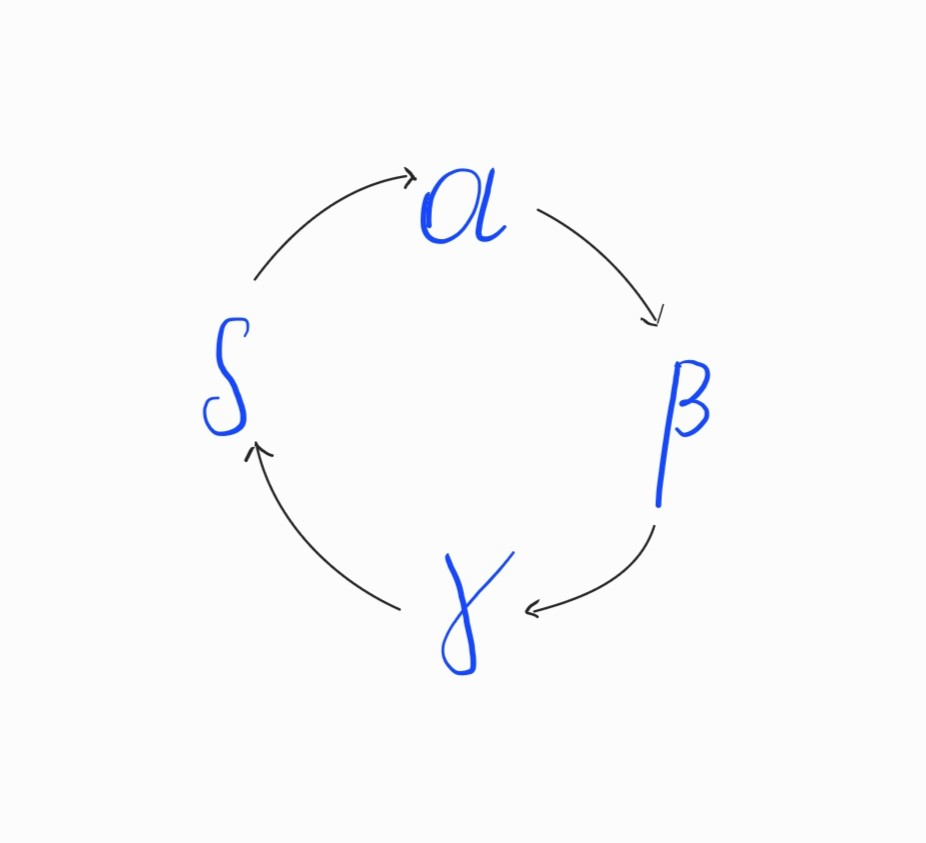
\includegraphics[width=5cm]{Immagini/Pari.jpg} }}%
    \qquad
    \subfloat[\centering Dispari]{{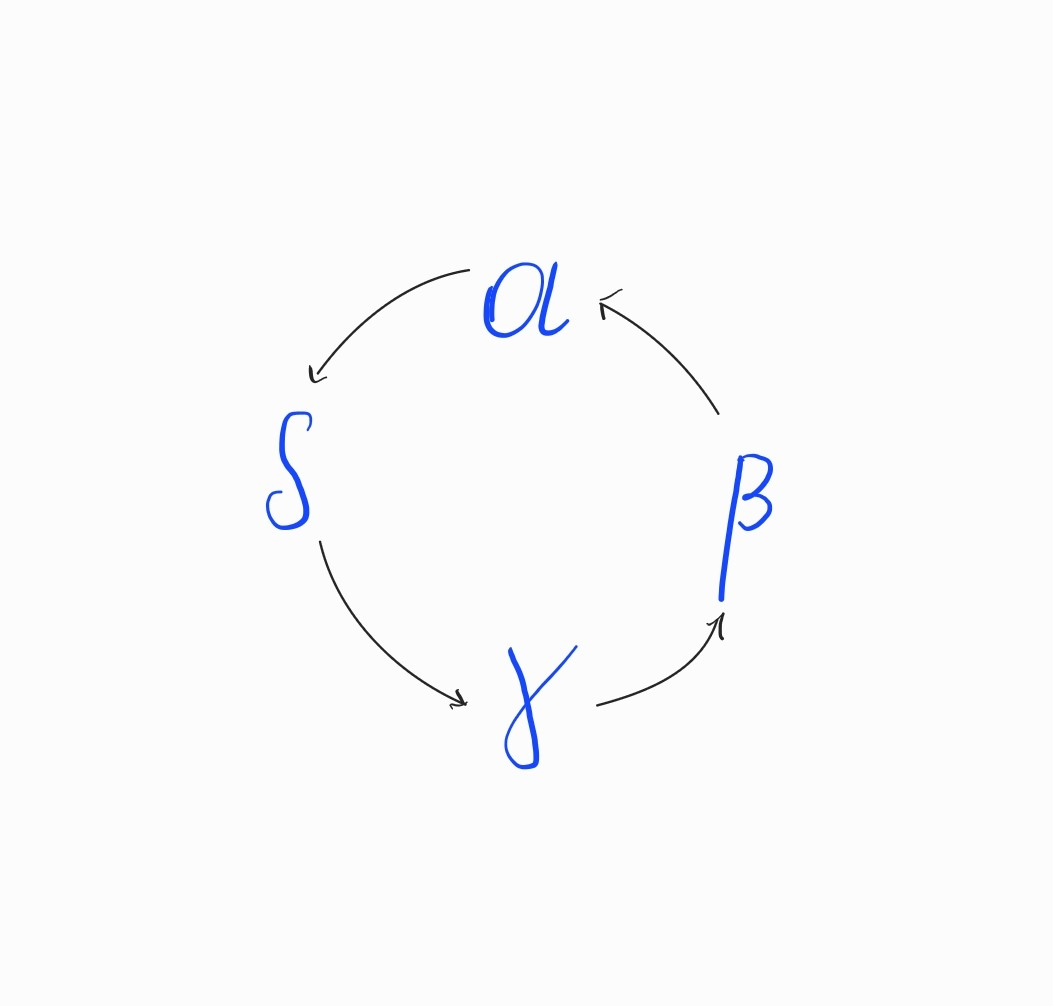
\includegraphics[width=5cm]{Immagini/Dispari.jpg} }}%
    \caption{Permutazioni}%
    \label{fig:permu}%
\end{figure}

Ora, possiamo verificare una proprietà dei vettori contravarianti e covarianti, ovvero \textit{abbassamento/innalzamento di indice}. Consideriamo il tensore $A^{\alpha}=(A^0, \Vec{A})$ di rango $(1,0)$, allora possiamo ottenere un vettore covariante operando:
\begin{equation*}
\eta\indices{_{\mu\alpha}}A^\alpha=B_\mu
\end{equation*}
ciò che avviene nell'algebra dei ranghi è $(0,2)\otimes(1,0)\rightarrow(1,2)\rightarrow(0,1)$. Sviluppando i conti si ottiene che $B_{\mu}=(B_0,B_1,B_2,B_3)=(A^0,-A^1,-A^2,-A^3)$, quindi sostanzialmente, in relatività ristretta, il passaggio da covariante a contravariante consiste nel cambio di segno delle tre componenti spaziali\footnote{In relatività generale non è così semplice.}.
Ovviamente si può fare l'operazione opposta usando la matrice metrica inversa.

Alla luce di ciò, possiamo definire la \textit{norma} di un vettore quadridimensionale come il prodotto scalare del vettore per il suo \say{reciproco in rango}, ovvero:  
\begin{equation*}
A^{\alpha}A_{\alpha}=A^0A_0+A^1A_1+A^2A_2+A^3A_3=A^0A^0-A^1A^1-A^2A^2-A^3A^3=(A^0)^2-|\vec{A}|^2
\end{equation*}
risulta evidente a questo punto come $ds^2$ sia la norma di un evento. Possiamo fare altri esempi, consideriamo il quadrivettore energia-impulso e la relazione di Einsten per un sistema in quiete ($\Vec{v}=0$):
\begin{equation*}
P^{\alpha}P_{\alpha}=\dfrac{E^2}{c^2}-|\vec{P}|^2=m^2c^2
\end{equation*}
tale norma sarà sicuramente maggiore di 0 (questo perché la massa è definita reale e positiva), quindi di genere tempo. Un altro esempio lo abbiamo se consideriamo il quadrigradiente covariante e contravariante:
\begin{equation}
\partial_\alpha=\dfrac{\partial }{\partial x^\alpha}=(\dfrac{1}{c}\dfrac{\partial }{\partial t},\Vec{\nabla}) \qquad \partial^\alpha=\dfrac{\partial }{\partial x_\alpha}=(\dfrac{1}{c}\dfrac{\partial }{\partial t},-\Vec{\nabla})
\end{equation}
possiamo ottenere l'operatore di D'Alembert\footnote{Ricordiamo che seguendo il formalismo tensoriale, esso, ci permette di dire che se una grandezza è uno scalare, allora è un invariante per trasformazioni di Lorentz.}:
\begin{equation}
\partial_\alpha\partial^\alpha=\dfrac{1}{c^2}\dfrac{\partial^2 }{{\partial t}^2}-{\nabla}^2
\end{equation}

Considerando, ora, la quadricorrente $J^\mu=(c\rho,\vec{j})$, possiamo definire, in generale, la \textit{quadridivergenza} come:
\begin{equation} \phantomsection \label{eq:eq_cont}
\partial_\mu J^\mu=\dfrac{\partial\rho }{{\partial t}}+\vec{\nabla}\Vec{j}
\end{equation}
ovviamente risulta essere uno scalare e la forma è quella di un'equazione di continuità.

Consideriamo l'operazione di integrazione in relatività ristretta. La varietà che si considera è quella di Minkowski, quindi la misura di integrazione dovrà essere quella di un evento infinitesimo:

\begin{equation}
\int d^4x=\int cdt d^3x
\end{equation}
inoltre, la misura, dovrà essere Lorentz invariante, possiamo mostrarlo rapidamente.
Considerando una trasformazione di Lorentz, avremo che, per il teorema del cambiamento di variabile, la misura si trasforma secondo:
\begin{equation}
  x^{\alpha}\xrightarrow[\text{}]{\text{T}}x'^{\alpha}=\Lambda\indices{^\alpha_\beta} x^{\beta} \qquad d^4x\xrightarrow[\text{}]{\text{T}}d^4x'=|J(x)|d^4x
\end{equation}
ove $J(x)=det\{ \dfrac{\partial x'^\alpha}{\partial x^\beta}\}=det\Lambda\indices{^\alpha_\beta}$ è il determinate dello jacobiano associato alla trasformazione, inoltre sappiamo che le trasformazioni di Lorentz possono essere proprie o improprie, quindi la conservazione dei volumi è garantita.


\subsection{Equazioni tensoriali}\label{sec:1.5}
Consideriamo due sistemi di riferimento inerziali, come in Fig.\ref{fig:TL}, ed ipotizziamo che in $S$ sia vera l'equazione tensoriale:
\begin{equation*}
    T\indices{^\alpha_\beta}=S\indices{^\alpha_\beta}
\end{equation*}
allora potrò riscrivere per il sistema $S'$:
\begin{equation*}
   T\indices{^'^\alpha_\beta} =\Lambda\indices{^\alpha_\mu}\Lambda\indices{_\beta^\nu}T\indices{^\mu_\nu}=\Lambda\indices{^\alpha_\mu}\Lambda\indices{_\beta^\nu}S\indices{^\mu_\nu}=S\indices{^'^\alpha_\beta}
\end{equation*}
concludiamo che se siamo in grado di scrivere leggi fisiche in formalismo tensoriale sappiamo, per costruzione, che queste saranno invarianti in forma per tutti i sistemi di riferimento inerziali. La convenienza di questo formalismo risiede proprio in questa proprietà, cioè che soddisfa in maniera del tutto naturale il primo postulato della relatività.

Alcune quantità fisiche fondamentali non sono tensori (per esempio velocità, accelerazione e forza), quindi per risolvere questo problema introdurremo quantità tensoriali che le rappresentino esaustivamente.


\subsection{Fondamenti di Meccanica Relativistica}\label{sec:1.6}
Consideriamo un sistema $S$ in quiete e un sistema $S'$ in moto vario. Quindi, l'osservatore in $S$, in un tempo $dt$, vedrà spostarsi $S'$ di una quantità $\sqrt{dx^2+dy^2+dz^2}$. Ci chiediamo che relazione c'è tra $dt$ e $dt'$. Per rispodnere usiamo gli intervalli invarianti, ricordando che rispetto a $S'$ lo spostamento sarà nullo:
\begin{equation*}
    {ds}^2=c^2{dt}^2-{dx}^2-{dy}^2-{dz}^2=c^2{dt'}^2-{dx'}^2-{dy'}^2-{dz'}^2=c^2{dt'}^2
\end{equation*}
    quindi definiamo il \textit{tempo proprio}, come:
\begin{equation}
    dt'=\dfrac{ds}{c}=dt\sqrt{1-\dfrac{{dx}^2+{dy}^2+{dz}^2}{c^2{dt}^2}}=dt\sqrt{1-\dfrac{{v}^2}{c^2}}=\dfrac{dt}{\gamma}
\end{equation}

Consideriamo la lunghezza di una traiettoria $\gamma$ nello spazio di Minkowski fissati due tempi $(t_f,t_i)$: 
\begin{equation*}
    \mathcal{L}(t_f-t_i)=\int_\gamma ds=\int_\gamma c\sqrt{1-\dfrac{v^2}{c^2}}dt
\end{equation*}
ovviamente l'integrale dipende dal percorso gamma, quindi da come l'oggetto si muove spaziotemporalmente. Se fossimo in $\mathbb{R}^3$ la risposta sarebbe che lungo la retta l'integrale è minimo, invece, poiché siamo in uno spazio con una geometria non euclidea, l'integrale, lungo una retta, è massimo. Infatti se consideriamo una particella a riposo il termine sotto radice è 1, mentre se la particella è in movimento il termine sotto radice sarà minore di 1, quindi complessivamente l'integrando sarà minore di c.

Definiamo il \textit{quadrivettore velocità} come la derivata di un quadrivettore posizione nel tempo proprio\footnote{Notiamo che la grandezza che ne risulta è adimensionale, non ostante ciò continueremo a chiamarla velocità.}:
\begin{equation}\phantomsection\label{eq:def_qvel}
    u^\alpha=\dfrac{dx^\alpha}{ds}
\end{equation}
le componenti della quadrivelocità saranno (considerando le definizioni di tempo proprio $ds=c\dfrac{dt}{\gamma}$) $u^0=\dfrac{dx^0}{ds}=\gamma$ e $\Vec{u}=\dfrac{d\vec{x}}{ds}=\dfrac{\vec{v}}{c}\gamma$. Dimostriamo che tale quadivettore ha norma 1\footnote{Quindi sarà di tipo tempo.}.
\begin{proof}
\begin{equation}
    \begin{gathered}\phantomsection\label{eq:Norm_Vel}
      {ds}^2=\eta\indices{_{ij}}dx^idx^j    \\
  1=\dfrac{{ds}^2}{{ds}^2}=\eta\indices{_{ij}}\dfrac{dx^i}{ds}\dfrac{dx^j}{ds}   \\
1=\eta\indices{_{ij}}u^iu^j=u_ju^j
\end{gathered}
\end{equation}

\end{proof}
Definiamo il \textit{quadrivettore accelerazione} come la derivata di un quadrivettore velocità nel tempo proprio:

\begin{equation}\label{eq:def_qacc}
    \omega^\alpha=\dfrac{du^\alpha}{ds}=\dfrac{d^2x^\alpha}{ds^2}
\end{equation}
le componenti della quadriaccelerazione saranno (considerando l'accelerazione classica $\Vec{a}=\dfrac{d\Vec{v}}{dt}$) $ \\\omega^0=\dfrac{\gamma^4}{c^3}\Vec{v}\Vec{a}$ e $u^i=\dfrac{\gamma^2}{c^2}[a^i+\dfrac{\gamma^2}{c^2}(\Vec{v}\Vec{a})v^i]$. Dimostriamo che quadrivelocità e quadriaccelerazione sono ortogonali (in senso lorentziano), per farlo partiamo il risultato precedente e differenziamo per $\dfrac{d}{ds}$:
\begin{proof}
\begin{equation}
        \begin{gathered}\phantomsection\label{eq:Orto_Vel_Acc}
      u_ju^j=1 \\
\eta\indices{_{ij}}\omega^iu^j=0 \\
\omega^iu_i=0
\end{gathered}
\end{equation}
\end{proof}
poiché il prodotto scalare è nullo, concludiamo che sono ortogonali.
Dimostriamo anche che la quadriaccelerazione è un vettore di tipo spazio, ossia che $\omega^\alpha\omega_\alpha<0$. 
 \begin{proof}
     Dall'ortogonalità so che:
\begin{gather*}
\omega^iu_i=0\\
\omega^0u^0-\Vec{\omega}\Vec{u}=0  \implies \omega^0=\dfrac{\Vec{\omega}\Vec{u}}{u^0}
\end{gather*}
sostituiamo nella norma di $\omega^\alpha$:
\begin{equation}
    \begin{gathered}\phantomsection\label{eq:seg_Acc}
      \omega_j\omega^j=(\omega^0)^2-|\vec{\omega}|^2=\left(\dfrac{\Vec{\omega}\Vec{u}}{u^0}\right) ^2 -|\vec{\omega}|^2 \\
\omega_j\omega^j=\left(\dfrac{\Vec{\omega}\Vec{u}}{u^0}\right)^2 -|\vec{\omega}|^2=\dfrac{\Vec{(\omega})^2(\Vec{u})^2\cos^2{\theta}}{(u^0)^2} -|\vec{\omega}|^2 \\
\omega_j\omega^j=-\dfrac{\Vec{(\omega})^2}{(u^0)^2}\left[(u^0)^2-|\vec{u}|^2\cos^2{\theta}\right]<0
\end{gathered}
\end{equation}

 \end{proof}
 ove $\theta$ è l'angolo compreso tra i vettori. La disuguaglianza finale deriva, banalmente, dal fatto che $u_ju^j=(u^0)^2-(\Vec{u})^2=1 $.
 
Introducendo l'impulso relativistico\footnote{Il motivo per cui l'impulso in relatività cambia definizione è che la relazione $\Vec{p}=m\Vec{v}$ non rispetta la conservazione (che deriva dall'omogeneità dello spazio) in tutti i sistemi di riferimento inerziali.}
\begin{equation}
    \Vec{p}=\dfrac{m\Vec{v}}{\sqrt{1-\dfrac{v^2}{c^2}}}
\end{equation}
il \textit{principio di inerzia}\footnote{Ricordiamo che, essendo una relazione vettoriale, essa rappresenta tre equazioni indipendenti.} assume la forma:
\begin{equation}\phantomsection\label{eq:princ_iner}
    \Vec{F}=\dfrac{d\Vec{p}}{dt}
\end{equation}
mentre il \textit{teorema delle forze vive}\footnote{Possiamo riscrivere il teorema delle forze vive in funzione di E poiché $T=E-mc^2$, ma il termine $mc^2$ è costante} rimane:
\begin{equation}\phantomsection\label{eq:teo_for_vive}
    \Vec{F}\Vec{v}=\dfrac{dT}{dt}=\dfrac{dE}{dt}
\end{equation}
L'idea di Minkowki fu quella di riunire queste quattro equazioni della dinamica relativistica in una sola equazione tensoriale. Definiamo il \textit{quadrimpulso}:
\begin{equation}\phantomsection\label{eq:def_quadimpul}
    P^\alpha=\left(\dfrac{E}{c},\Vec{p}\right)=mcu^\alpha
\end{equation}
e la relazione che le unifica è:
\begin{equation}\phantomsection\label{eq:quad_for}
   \dfrac{dP^\alpha}{ds}=\mathcal{F}^\alpha=\left(\mathcal{F}^0,\Vec{\mathcal{F}}\right)
\end{equation}
ove $ds$ è il tempo proprio e $\mathcal{F}^\alpha$ è datta \textit{quadriforza di Minkowski}.
Possiamo ricavare le componenti della forza di Minkowski, semplicemente: 
\begin{gather*}
   \mathcal{F}^0=\dfrac{dp^0}{ds}=\dfrac{1}{c}\dfrac{dE}{dt}\dfrac{dt}{ds}=\dfrac{1}{c}\Vec{F}\Vec{v}\dfrac{\gamma}{c}\\
   \Vec{\mathcal{F}}=\dfrac{d\Vec{p}}{ds}=\dfrac{d\Vec{p}}{dt}\dfrac{dt}{ds}=\dfrac{\gamma}{c}\Vec{F}
\end{gather*}
Dimostriamo rapidamente che $\mathcal{F}^0$ è dipendente da $\Vec{\mathcal{F}}$. Sappiamo che:
\begin{equation*}
  \mathcal{F}^\alpha=\dfrac{dP^\alpha}{ds}=mc\dfrac{du^\alpha}{ds}=mc\omega^\alpha\\
  \end{equation*}
   quindi dall'ortogonalià di $\omega^\alpha$ e $u^\alpha$:
   \begin{equation*}
        \mathcal{F}^\alpha u^\alpha= \mathcal{F}^0u^0-\Vec{\mathcal{F}}\Vec{u}=0  \implies \mathcal{F}^0=\dfrac{\Vec{\mathcal{F}}\Vec{u}}{u^0} 
   \end{equation*}
   Ricordiamo, infine, che quanto detto finora non rappresenta una nuova fisica, ma solamente un nuovo formalismo che risulta, però, necessario per avere una maggiore agilità nei calcoli e per sviluppare calcoli più complessi.
   \subsection{Coordinate di Rindler}\label{sec:1.7}
Vogliamo definire un moto uniformemente accelerato in relatività ristretta. Ovviamente la definizione dovrà essere valida per ogni sistema di riferimento, quindi indipendente da quest'ultimo, in maniera da essere conforme al primo postulato. Tale definizione seguita dalla norma della quadriaccelerazione:
\begin{equation}\label{eq:Unif_Acc}
    \omega_j\omega^j=-g^2
\end{equation}
ove $g$ è uno scalare costante, per rispettare l'uniformità. Per semplicità consideriamo il caso in cui il moto avvenga solo lungo x. Ciò che conosciamo sono le relazioni \eqref{eq:Norm_Vel}, \eqref{eq:Orto_Vel_Acc} e \eqref{eq:Unif_Acc} che riscriviamo nella forma:

\begin{equation}\label{eq:Cond_Rindler}
    \begin{cases}
      (u^0)^2-(u^1)^2=1
             \\
     \omega^0u^0-\omega^1 u^1=0
              \\
     (\omega^0)^2-(\omega^1)^2=-g^2
    \end{cases}\,
\end{equation}
Dalla seconda equazione ricaviamo $\omega^0=\dfrac{\omega^1 u^1}{u^0}$, che sostituito nella terza:
\begin{gather*}
\left(\dfrac{\omega^1 u^1}{u^0}\right)^2-(\omega^1)^2=-g^2\\
\left(\dfrac{\omega^1}{u^0}\right)^2[(u^1)^2-(u^0)^2]=-g^2
    \end{gather*}
    Nel termine tra parentesi quadre riconosciamo la prima equazione delle \eqref{eq:Cond_Rindler} cambiata di segno. Sostituendo e cambiando di segno possiamo esplicitare $\omega^1$, per poi sostituirlo a sua volta in $\omega^0$. Infine, considerando la definizione di quadriaccelezaione otteniamo due equazioni differenziali:
    \begin{equation}\label{eq:Cond_Cost}
   \begin{gathered}
\left(\dfrac{\omega^1}{u^0}\right)^2=g^2 \implies
   \begin{cases}
      \omega^1=gu^0=\dfrac{du^1}{ds}
      \\
     \omega^0=gu^1=\dfrac{du^0}{ds}
      \end{cases}\, 
    \end{gathered} 
\end{equation}
Alla luce di quanto abbiamo appena ottenuto consideriamo la derivata seconda rispetto al tempo proprio di $u^0$ e $u^1$.
\begin{equation}
   \begin{cases}
    \dfrac{d^2u^1}{{ds}^2}=g\dfrac{du^0}{ds}=g^2u^1
      \\
      \\
    \dfrac{d^2u^0}{{ds}^2}=g\dfrac{du^1}{ds}=g^2u^0
      \end{cases}\, 
\end{equation}
Le soluzioni generali di queste equazioni differenziali al secondo ordine sono:
\begin{equation*}
   \begin{cases}
      u^1=Ae^{gs}+Be^{-gs}
      \\
     u^0=Ce^{gs}+De^{-gs}
      \end{cases}\, 
\end{equation*}
Tuttavia sappiamo che per il moto considerato quattro costanti di integrazioni sono troppe, difatti consideriamo una delle \eqref{eq:Cond_Cost} come condizione per determinare la dipendenza tra le costanti:
 \begin{equation*}
     \dfrac{du^0}{ds}=gu^1 \implies gAe^{gs}-gBe^{-gs}=gCe^{gs}+gDe^{-gs}
\implies A=C \land B=-D
\end{equation*} quindi considerano $A$ e $B$:
\begin{equation*}
   \begin{cases}
      u^1=Ae^{gs}+Be^{-gs}
      \\
     u^0=Ae^{gs}-Be^{-gs}
      \end{cases}\, 
\end{equation*}
Poniamo le condizioni iniziali $s=0$, $v=0$ e consideriamo la quadrivelocità $u^\alpha=(\gamma,\dfrac{\Vec{v}}{c}\gamma)=(1,0)$, quindi otteniamo:
\begin{equation}
   \begin{cases}
     u^1=0=A+B
      \\
     u^0=1=A-B 
      \end{cases}\, 
      \implies
    \begin{cases}
      A=\dfrac{1}{2}
      \\
      \\
      B=-\dfrac{1}{2}
      \end{cases}\, 
\end{equation}
sostituendo e ricordando le identità $\cosh{x}=\dfrac{e^x+e^{-x}}{2}$, $\sinh{x}=\dfrac{e^x-e^{-x}}{2}$:
\begin{equation}
   \begin{cases}
      u^1=\dfrac{1}{2} e^{gs}-\dfrac{1}{2}e^{-gs}=\sinh{gs}
      \\
      \\
     u^0=\dfrac{1}{2}e^{gs}+\dfrac{1}{2}e^{-gs}=\cosh{gs}
      \end{cases}\, 
\end{equation}
Dalla definizione di quadrivelocità \eqref{eq:def_qvel}, possiamo integrare ed ottenere:
\begin{equation}\label{eq:solu_rindler}
   \begin{cases}
      x^1=\dfrac{1}{g}\cosh{gs}
      \\
      \\
     x^0=\dfrac{1}{g}\sinh{gs}
      \end{cases}\, 
\end{equation}
Queste soluzioni del moto ci permettono di scrivere la legge del moto uniformemente accelerato in relatività ristretta:
\begin{equation}
    (x^1)^2-(x^0)^2=\dfrac{1}{g^2}
\end{equation}
Tale funzione nello spazio di Minkowski rappresenta un iperbole\footnote{Ricordiamo, per completezza, che in meccanica classica il moto uniformemente accelerato è rappresentato funzionalmente da una parabola.}, come mostrato in Fig.\ref{fig:MUA}

\begin{figure}[h]
    \centering
    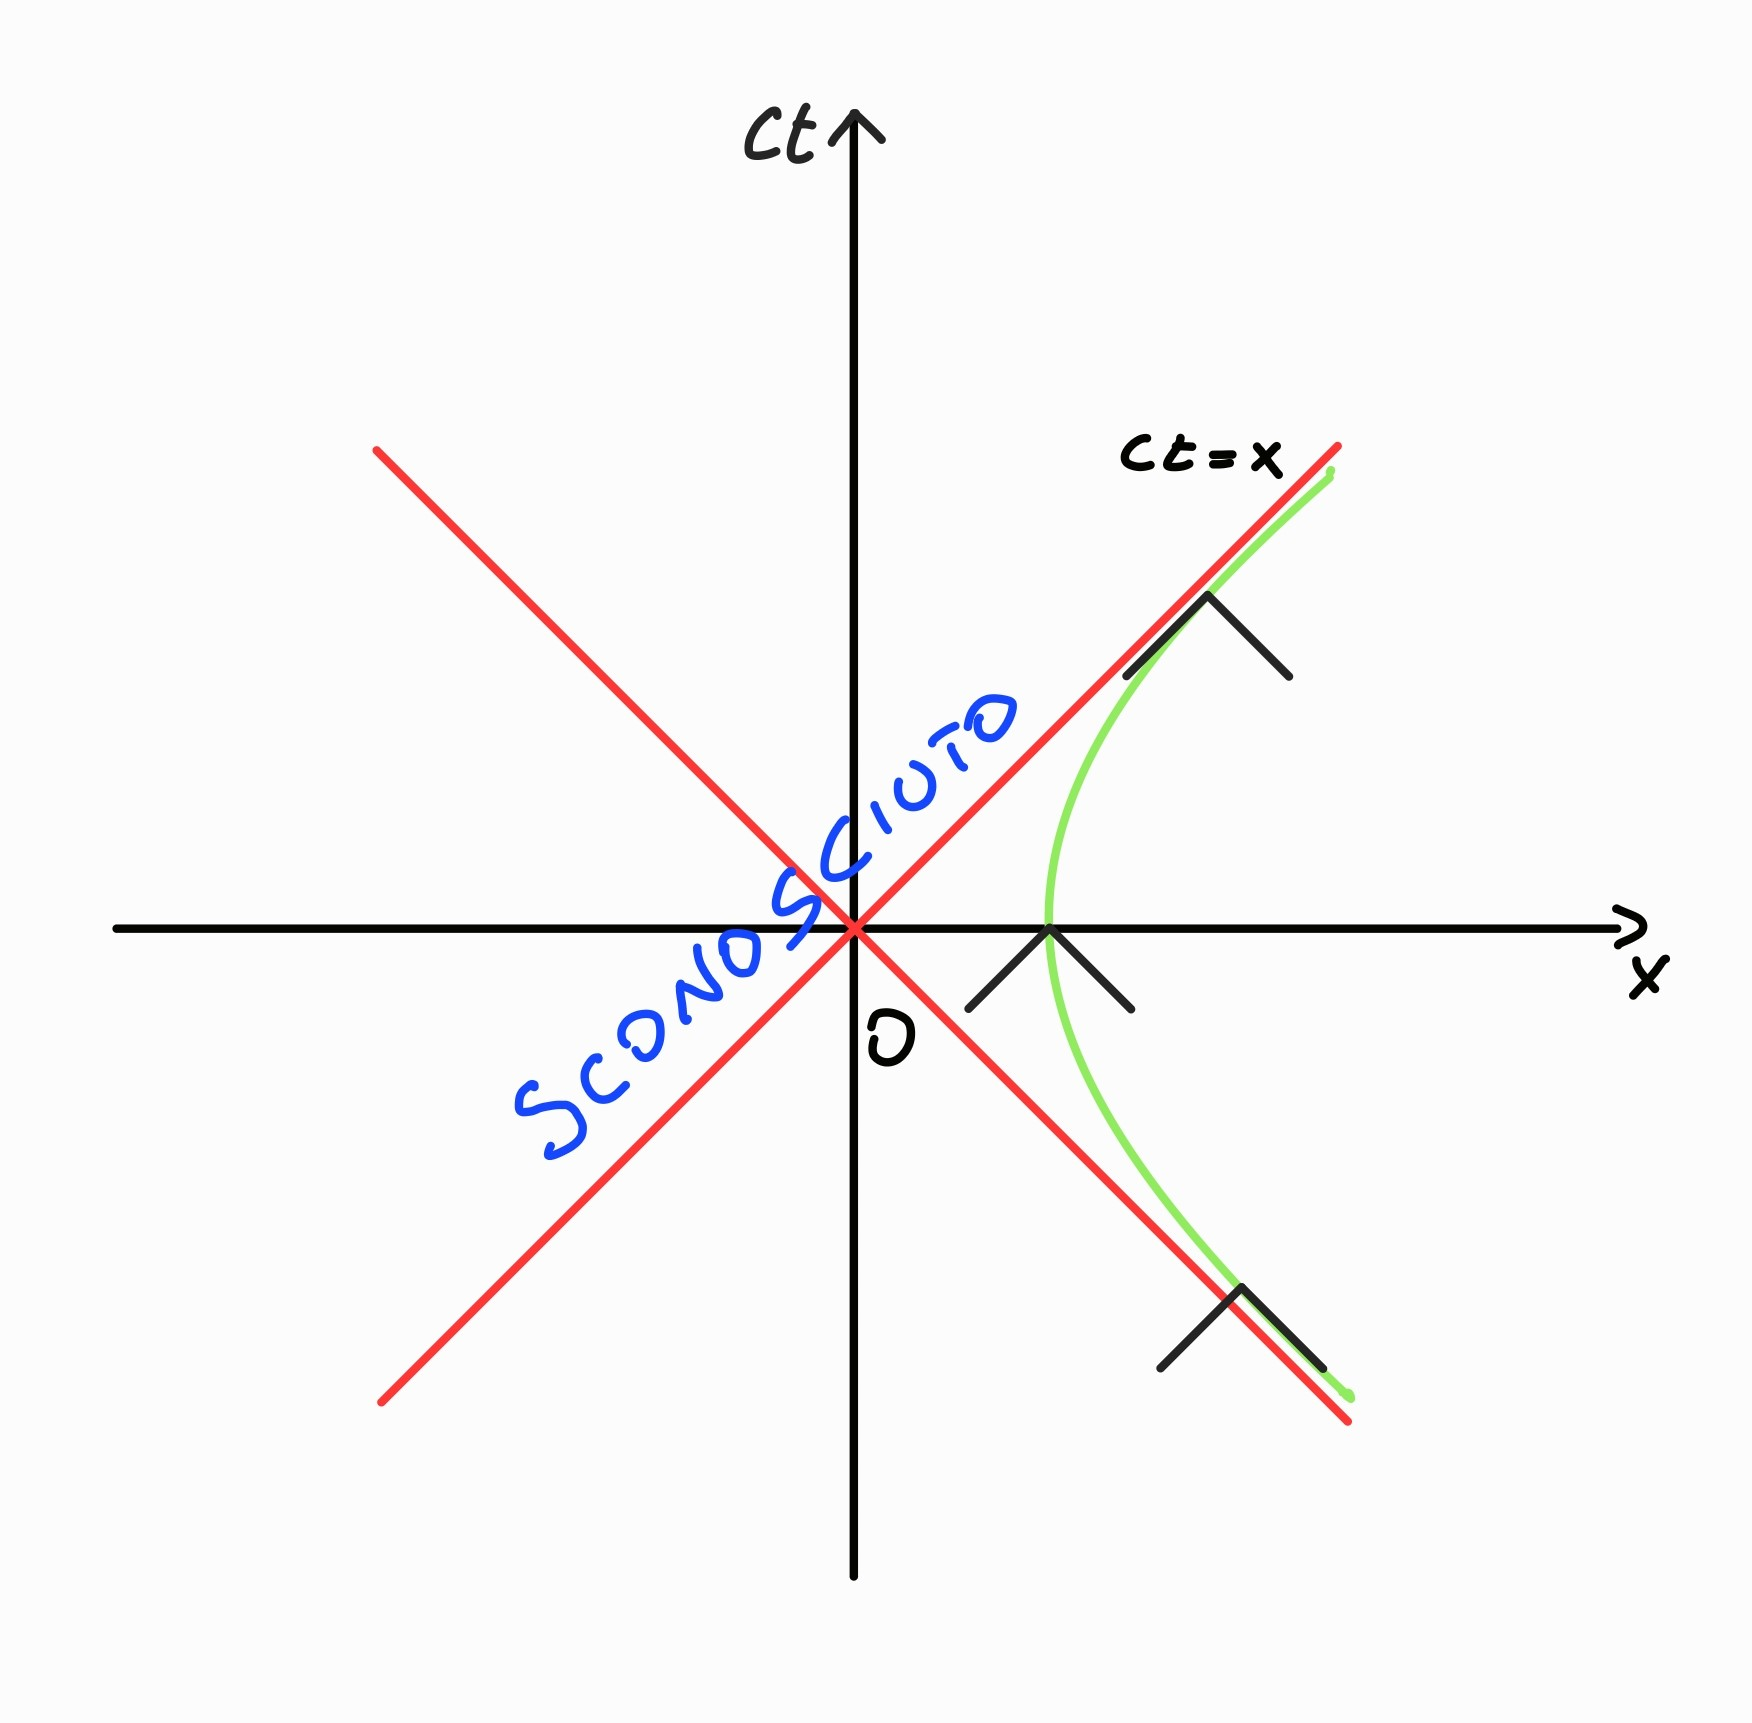
\includegraphics[width=0.395\textwidth]{Immagini/Rindler.jpg}
    \caption{ Moto uniformemente accelerato nello spazio di Minkowski}
    \label{fig:MUA}
\end{figure}
Possiamo, inoltre, dire che un osservatore che si muove di moto uniformemente accelerato non è un osservatore della relatività ristretta; la fisica vista da tale osservatore non è la fisica vista da un osservatore inerziale. Come mostrato in figura, nell'ipotesi che l'osservatore sia accelerato indefinitamente, i coni di luce di un osservatore non inerziale non superano mai la bisettrice del primo e terzo quadrante, quella regione dello spazio tempo gli è perciò preclusa. 

Un simile osservatore accelerato viene detto \textit{osservatore di Rindler}. Possiamo definire un cambio di coordinate, che viene detto \textit{trasformazione di Rindler}\footnote{Ovviamente non è una trasformazione di Lorentz perché stiamo passando da un osservatore inerziale ad uno non inerziale}:
\begin{equation}
  (ct,x)\xrightarrow[\text{}]{\text{R}}(\xi, \eta) \quad : \quad
\begin{cases}
      ct=\xi \sinh{(k\eta)}
      \\
      \\
     x=\xi \cosh{(k\eta)}
      \end{cases}\, 
\end{equation}
ove $k$ è una fase generica. In tali coordinate l'intervallo non è invariante e assume la forma:
\begin{equation*}
    ds^2=c^2dt^2-dx^2=(k\xi)^2d\eta^2-d\xi^2  
\end{equation*}
Mentre la legge del moto diventa:
\begin{equation}
    (x)^2-(ct)^2=\xi^2
\end{equation}